\documentclass[11pt, letterpaper]{article}

\usepackage[T1]{fontenc}
\usepackage{lmodern}
\usepackage{microtype}
\usepackage{amsmath}
\usepackage{booktabs}
\usepackage{multirow}
\usepackage{geometry}
\geometry{margin=1in}
\usepackage{pgfplots}
\pgfplotsset{compat=1.17}
\usepackage{xcolor}
\usepackage{hyperref}
\hypersetup{colorlinks=true, linkcolor=blue!50!black, urlcolor=blue!50!black, citecolor=blue!50!black}

\newcommand{\hit}{\mathrm{Hit@3}}
\newcommand{\code}[1]{\texttt{#1}}

\title{\textbf{The Top-$K$ Candidate-Depth Anomaly in Hybrid Code Search:\\Additive Path Boosts, Not Semantic Noise}}
\author{B. Madusha R. Perera\\ \href{https://github.com/maduperera/Miru_}{\code{github.com/maduperera/Miru\_}}}
\date{\today}

\begin{document}
\maketitle

\begin{abstract}
Hybrid code-search engines commonly fetch a deep candidate pool and truncate it to the few results an agent or
LLM will read, on the assumption that a deeper pool can only help. We test this assumption on Miru
(\code{@takara-ai/miru-code} v1.12.2), a BM25 + dense hybrid engine that fetches $5K$ candidates per retriever before
rank fusion, using 150 identifier-lookup queries over \code{kubernetes/client-go} (13{,}471 chunks). Requesting
$K{=}3$ instead of $K{=}50$-then-truncating raises $\hit$ from 76.0\% to 83.3\% (+7.3 points, 95\% CI [3.3, 12.0];
11 wins, 0 losses; exact sign test $p<0.001$) and lowers median search latency by 33\%. Using a reimplementation of
Miru's search that we verify to be output-identical on all queries, we isolate the cause. The effect is entirely a
function of candidate depth (final truncation contributes exactly zero), it is driven by the depth of the BM25 list
(deepening the dense list alone has no significant effect), and it disappears when Miru's additive file-path
\emph{stem boost} is disabled. The depth penalty grows monotonically with the boost strength, from 0 points at
$\beta\le0.25$ to +7.3 at Miru's default $\beta{=}0.75$ and +27.3 at $\beta{=}1.5$. All 33 results that displaced a
correct answer under deep fetching carried this boost, and 28 of them were files whose name equals a single query
word (e.g.\ \code{interface.go}, \code{role.go}). The anomaly is therefore an interaction between pool depth and a
post-fusion boost whose magnitude rivals the fused relevance scores, not semantic noise from the vector index.
Results use a local MiniLM embedder as a stand-in for Miru's production DS1 model.
\end{abstract}

%=====================================================================================================================
\section{Introduction}
Coding agents retrieve a handful of code chunks per step and place them in a constrained context window, so the
top few results of the underlying search engine largely determine whether the agent sees the right definition.
Hybrid retrieval, which fuses lexical (BM25~\cite{robertson2009bm25}) and dense~\cite{reimers2019sbert} signals, is
the usual design, and a common integration pattern is to request a generous result count (e.g.\ $K{=}50$) and
truncate client-side to the top 3. The implicit assumption is that a deeper pool gives the ranker more to choose from
and so cannot make the top of the list worse.

We show that, in Miru, it does, and we identify why. Miru, like many hybrid engines, scales the number of candidates
it pulls from each retriever with the requested $K$. Changing $K$ therefore changes the \emph{inputs} to fusion and
re-ranking, not only how many outputs are returned. Our contributions are:
\begin{enumerate}
  \item A reproducible benchmark (open source, MIT) showing a +7.3-point $\hit$ gain and 33\% lower median latency
        from requesting $K{=}3$ rather than $K{=}50$ and truncating (\S\ref{sec:headline}).
  \item A fidelity-verified, split-depth reimplementation of Miru's search that lets the dense and BM25 candidate
        depths, the final cut-off, the fusion weight and each post-fusion stage be varied independently
        (\S\ref{sec:setup}).
  \item A causal decomposition through six controlled experiments: the effect is pure candidate depth
        (\S\ref{sec:factorial}), is driven by BM25 depth rather than dense depth (\S\ref{sec:grid}), vanishes without the
        path-stem boost (\S\ref{sec:stages}), and scales with the boost's strength (\S\ref{sec:dose}).
  \item A per-query anatomy of every displaced answer, showing two distinct pathways by which depth helps a boosted
        distractor (\S\ref{sec:anatomy}).
\end{enumerate}

%=====================================================================================================================
\section{System Under Study}\label{sec:system}
We describe Miru's \code{hybridSearch}~\cite{miru} as implemented in \code{src/search.ts} and \code{src/ranking/} of v1.12.2.
For a query $q$ and requested result count $K$:

\paragraph{1. Candidate generation.} Every chunk is scored by BM25 and by dense cosine similarity. The top
$d = mK$ chunks of \emph{each} list are kept, where $m$ is \code{MIRU\_RANK\_CANDIDATE\_MULTIPLIER} (default 5;
location-style queries use 10, but none of our queries trigger this). For $K{=}3$, $d{=}15$; for $K{=}50$, $d{=}250$.
Note that full-corpus scoring happens regardless of $K$; only the selected depth changes.

\paragraph{2. Rank fusion.} Each list is converted to reciprocal-rank scores~\cite{cormack2009rrf} with $k{=}10$ and
combined with a fusion weight $\alpha$ (0.25 for natural-language queries, 0.30 for symbol-like queries):
\begin{equation}
  f(c) \;=\; \frac{\alpha}{k + r_{\mathrm{dense}}(c)} \;+\; \frac{1-\alpha}{k + r_{\mathrm{bm25}}(c)},
  \label{eq:fusion}
\end{equation}
where a chunk absent from a list contributes 0 for that term. Fused scores are therefore small and tightly packed:
the maximum possible value is $1/11 \approx 0.091$.

\paragraph{3. Path-stem boosts.} For natural-language queries, Miru adds two boosts to every chunk in the pool.
Let $M = \max_c f(c)$ over the pool, $Q$ the query keywords, and $\beta$ = \code{MIRU\_RANK\_EXACT\_STEM\_BOOST}
(default 0.75). A partial boost of $\beta M \cdot \rho(c)$ is added, where $\rho(c)$ is the fraction of query keywords
matching (exactly or by prefix) a token of the chunk's file stem or parent directory. A further exact boost of
$\beta M$ is added if the file stem equals any single query keyword:
\begin{equation}
  s(c) \;=\; f(c) \;+\; \beta M\,\rho(c) \;+\; \beta M\,\mathbb{1}\!\left[\mathrm{stem}(c)\in Q\right].
  \label{eq:boost}
\end{equation}
Both boosts are \emph{additive} and scaled by the pool maximum, so a single exact-stem match is worth $0.75M$, which is
comparable to the entire fused score of the best candidate.

\paragraph{4. Re-ranking.} Path penalties (tests, examples, compatibility directories) and a per-file saturation
decay are applied, and the top $K$ chunks are returned.

%=====================================================================================================================
\section{Experimental Setup}\label{sec:setup}
\paragraph{Corpus.} \code{kubernetes/client-go} at commit \code{2761958}, indexed by Miru into 13{,}471 chunks.

\paragraph{Queries and metric.} 150 frozen queries. Each is a Go identifier split into lowercase words (e.g.\
\code{LeaseCandidateInterface} $\to$ ``lease candidate interface'') and is paired with every file that defines the
identifier (at least two per query; a test verifies each file defines it). A query is a hit if any defining file
appears among the top 3 results ($\hit$). We also report MRR@3.

\paragraph{Embedder.} Miru's production embedder (DS1) requires an API key we did not have. We use
\code{all-MiniLM-L6-v2}~\cite{wang2020minilm} truncated to 256 dimensions and re-normalised to match DS1's shape.
Query vectors are precomputed and injected, so every configuration is deterministic.

\paragraph{Split-depth harness.} To vary the two candidate depths independently, we reimplemented
\code{hybridSearch} line for line using Miru's own exported ranking functions, changing only the single depth $mK$
into separate dense and BM25 depths $(d_{\mathrm{dense}}, d_{\mathrm{bm25}})$. \textbf{Fidelity check:} with both
depths set to $mK$, the reimplementation's ranked output (file and start line) is identical to
\code{MiruIndex.search} on 150/150 queries at each of $K\in\{3,5,50\}$.

\paragraph{Statistics.} Proportions carry Wilson 95\% intervals~\cite{wilson1927}. Paired comparisons use the exact
two-sided sign test on discordant queries and a paired percentile bootstrap (10{,}000 resamples, fixed seed) for the
95\% CI of the difference~\cite{efron1993bootstrap}. Latency is measured on the real \code{MiruIndex.search}: one
warm-up call, then 5 repetitions per arm with arm order rotated across queries; we report the per-query median,
summarised as p50 and p95.

%=====================================================================================================================
\section{Results}

\subsection{Headline: requesting fewer results is more accurate and faster}\label{sec:headline}
\begin{table}[htbp]
\centering\small
\caption{End-to-end benchmark on \code{MiruIndex.search} ($n{=}150$). $\Delta$ and W/L are relative to Legacy.}
\label{tab:headline}
\begin{tabular}{@{}lrrrrrr@{}}
\toprule
Configuration & Depth/list & $\hit$ [95\% CI] & $\Delta$ [95\% CI] & W/L ($p$) & p50 ms & p95 ms \\
\midrule
Legacy ($K{=}50$, truncate to 3) & 250 & 76.0 [68.6, 82.1] & --- & --- & 31.5 & 39.7 \\
Mid-bound ($K{=}5$, truncate to 3) & 25 & 79.3 [72.2, 85.0] & +3.3 [0.7, 6.7] & 5/0 (0.063) & 21.6 & 30.6 \\
Optimized ($K{=}3$) & 15 & \textbf{83.3} [76.6, 88.4] & \textbf{+7.3} [3.3, 12.0] & 11/0 ($<$0.001) & \textbf{21.2} & \textbf{30.6} \\
\bottomrule
\end{tabular}
\end{table}

Table~\ref{tab:headline} shows that requesting $K{=}3$ fixes 11 queries Legacy misses and breaks none. MRR@3 rises
from 0.692 to 0.770. The fused candidate pool shrinks from a mean of 401 to 26 unique chunks (93.5\% fewer), but median
latency falls by only 33\%, because full-corpus BM25 and dense scoring is paid regardless of $K$.

\subsection{It is candidate depth, not truncation}\label{sec:factorial}
A $2\times2$ factorial crosses candidate depth (15 vs.\ 250 per list) with the final re-ranking cut-off (3 vs.\ 50,
always reading the first 3). $\hit$ is 83.3\% at depth 15 and 76.0\% at depth 250 \emph{for both cut-offs}; the cut-off
changes no query's outcome (0 wins, 0 losses at either depth). As an independent check on the unmodified engine,
running \code{MiruIndex.search} with $K{=}3$ but $m{=}50$ (150 per list, Miru's maximum) returns the same top-3 files as
Legacy on 146/150 queries, with identical $\hit$ (114/150).

\subsection{Accuracy follows an inverted U in depth}\label{sec:sweep}
\begin{figure}[htbp]
\centering
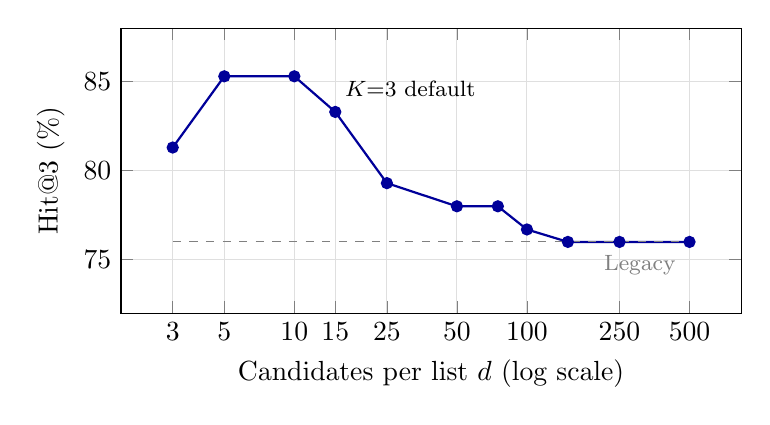
\begin{tikzpicture}
\begin{axis}[width=0.78\linewidth, height=5.2cm, xmode=log, log basis x=10,
  xlabel={Candidates per list $d$ (log scale)}, ylabel={$\hit$ (\%)}, ymin=72, ymax=88,
  xtick={3,5,10,15,25,50,100,250,500}, xticklabels={3,5,10,15,25,50,100,250,500},
  grid=major, grid style={gray!25}, mark size=1.8pt]
\addplot[thick, blue!60!black, mark=*] coordinates {
  (3,81.3) (5,85.3) (10,85.3) (15,83.3) (25,79.3) (50,78.0) (75,78.0) (100,76.7) (150,76.0) (250,76.0) (500,76.0)};
\addplot[dashed, gray] coordinates {(3,76.0) (500,76.0)};
\node[anchor=south west, font=\footnotesize] at (axis cs:15,83.6) {$K{=}3$ default};
\node[anchor=north east, font=\footnotesize, gray] at (axis cs:480,75.8) {Legacy};
\end{axis}
\end{tikzpicture}
\caption{Symmetric depth sweep (same depth for both lists, first 3 results scored).}
\label{fig:sweep}
\end{figure}

Figure~\ref{fig:sweep} sweeps a common depth $d$ for both lists. Accuracy peaks at $d\in\{5,10\}$ (85.3\%, +9.3
points over $d{=}250$, 14/0, $p<0.001$), declines monotonically to 76.0\% by $d{=}150$, and stays flat beyond.
Very shallow pools also hurt ($d{=}3$: 81.3\%, 12 wins / 4 losses against $d{=}250$), as the correct chunk sometimes
falls outside both lists. Miru's default for $K{=}3$ ($d{=}15$) sits just past the optimum.

\subsection{The BM25 list, not the dense list, carries the effect}\label{sec:grid}
\begin{table}[htbp]
\centering\small
\caption{Left: $\hit$ (\%) over the dense $\times$ BM25 depth grid. Right: effect of deepening one list from 15 to 250
with the other fixed at 75 (shallow minus deep; positive means deepening hurts).}
\label{tab:grid}
\begin{tabular}{@{}lrrrrr@{}}
\toprule
 & \multicolumn{5}{c}{BM25 depth} \\
\cmidrule(l){2-6}
Dense depth & 15 & 30 & 75 & 150 & 250 \\
\midrule
15  & 83.3 & 79.3 & 78.0 & 77.3 & 77.3 \\
30  & 82.7 & 79.3 & 77.3 & 76.7 & 76.7 \\
75  & 83.3 & 80.0 & 78.0 & 76.7 & 76.0 \\
150 & 83.3 & 80.0 & 78.0 & 76.0 & 76.0 \\
250 & 83.3 & 80.0 & 78.0 & 76.0 & 76.0 \\
\bottomrule
\end{tabular}
\hspace{1.2em}
\begin{tabular}{@{}lrr@{}}
\toprule
Deepen only & $\Delta$ [95\% CI] & W/L ($p$) \\
\midrule
BM25  & +7.3 [3.3, 12.0] & 11/0 ($<$0.001) \\
Dense & \phantom{+}0.0 [$-$2.0, 2.0] & 1/1 (1.000) \\
\bottomrule
\end{tabular}
\end{table}

Table~\ref{tab:grid} varies the two depths independently. Reading down any column (deepening the dense list) barely
changes accuracy; reading along any row (deepening BM25) reproduces almost the full effect. Across all five fixed
levels of the other list, deepening BM25 from 15 to 250 costs 6.0--7.3 points (all $p\le0.004$), while deepening the
dense list changes $\hit$ by $-0.7$ to $+1.3$ points (all $p\ge0.5$). This rules out the hypothesis that semantic
noise from the vector index's long tail causes the anomaly.

\subsection{The post-fusion stem boost is necessary for the effect}\label{sec:stages}
\begin{table}[htbp]
\centering\small
\caption{Stage and fusion-weight ablations at depth 15 vs.\ 250 per list (first 3 results scored).}
\label{tab:stages}
\begin{tabular}{@{}lrrrr@{}}
\toprule
Pipeline variant & Depth 15 & Depth 250 & $\Delta$ [95\% CI] & W/L ($p$) \\
\midrule
Full Miru pipeline & 83.3 & 76.0 & +7.3 [3.3, 12.0] & 11/0 ($<$0.001) \\
No path-stem boosts ($\beta{=}0$) & 86.0 & 86.0 & 0.0 [0.0, 0.0] & 0/0 (1.000) \\
No path penalties & 82.7 & 75.3 & +7.3 [3.3, 12.0] & 11/0 ($<$0.001) \\
Fusion only (no boosts, no re-rank) & 85.3 & 84.7 & +0.7 [0.0, 2.0] & 1/0 (1.000) \\
\midrule
$\alpha = 0$ (BM25 weight only) & 84.7 & 78.0 & +6.7 [2.7, 10.7] & 10/0 (0.002) \\
$\alpha = 0.5$ & 75.3 & 69.3 & +6.0 [1.3, 10.7] & 11/2 (0.022) \\
$\alpha = 1$ (dense weight only) & 52.0 & 46.0 & +6.0 [2.7, 10.0] & 9/0 (0.004) \\
\bottomrule
\end{tabular}
\end{table}

Table~\ref{tab:stages} removes one stage at a time. Disabling the path-stem boosts eliminates the depth effect
entirely: no query changes outcome between the two depths. Removing all post-fusion processing leaves a negligible,
non-significant residue (+0.7). Path penalties are irrelevant. The fusion weight does not matter either: the depth
penalty persists at $\alpha{=}0$, at $\alpha{=}0.5$, and even at $\alpha{=}1$, where BM25 contributes nothing to the
fused score. This last case is informative. With $\alpha{=}1$, BM25-only candidates still enter the pool, with a fused
score of exactly zero, and the boost of Eq.~\eqref{eq:boost} alone can lift them into the top 3.

\subsection{Dose-response: the depth penalty scales with boost strength}\label{sec:dose}
\begin{figure}[htbp]
\centering
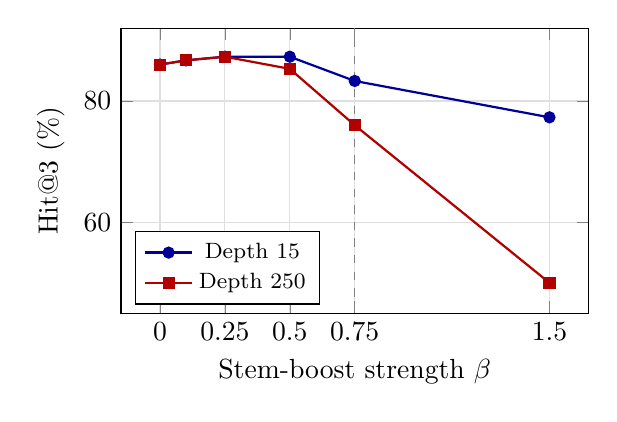
\begin{tikzpicture}
\begin{axis}[width=0.62\linewidth, height=5.2cm, xlabel={Stem-boost strength $\beta$}, ylabel={$\hit$ (\%)},
  ymin=45, ymax=92, xtick={0,0.25,0.5,0.75,1.5}, xticklabels={0,0.25,0.5,0.75,1.5},
  legend pos=south west, legend style={font=\footnotesize}, grid=major, grid style={gray!25}, mark size=1.8pt]
\addplot[thick, blue!60!black, mark=*] coordinates {(0,86.0) (0.1,86.7) (0.25,87.3) (0.5,87.3) (0.75,83.3) (1.5,77.3)};
\addplot[thick, red!70!black, mark=square*] coordinates {(0,86.0) (0.1,86.7) (0.25,87.3) (0.5,85.3) (0.75,76.0) (1.5,50.0)};
\addplot[dashed, gray] coordinates {(0.75,45) (0.75,92)};
\legend{Depth 15, Depth 250}
\end{axis}
\end{tikzpicture}
\caption{$\hit$ vs.\ stem-boost strength at both depths. The dashed line is Miru's default ($\beta{=}0.75$).}
\label{fig:dose}
\end{figure}

If the boost causes the anomaly, the depth penalty should grow with $\beta$. It does, monotonically (Figure~\ref{fig:dose}):
the penalty is 0 points for $\beta\in\{0, 0.1, 0.25\}$, +2.0 at 0.5 (3/0, n.s.), +7.3 at 0.75 (11/0, $p<0.001$), and
+27.3 at 1.5 (41/0, $p<0.001$, 95\% CI [20.0, 34.7]). Shallow pools are far more robust to the boost (83.3\% vs.\
50.0\% at $\beta{=}1.5$) because they contain fewer boostable distractors.

\subsection{Anatomy of a displaced answer}\label{sec:anatomy}
We traced every query that Legacy misses and Optimized hits (11 queries), recording each candidate's list ranks,
fused score $f$, and boost $s-f$. Legacy's top 3 on these queries contains 33 results, all of which outrank every
correct file.

\begin{itemize}
  \item \textbf{All 33 carry a path-stem boost.} In 28, the file name equals a single query word: \code{interface.go}
        (8), \code{role.go} (8), \code{eviction.go} (3), \code{scale.go} (3), \code{event.go} (3),
        \code{endpoint.go} (2), \code{pod.go} (1). These generic names recur in every API group and version of
        \code{client-go}.
  \item \textbf{The boost dominates relevance.} The median displacing result has fused score 0.028 but receives a boost
        of 0.080 (2.8$\times$), whereas the median correct file receives 0.019. Correct files often have compound stems
        (e.g.\ \code{storageclass.go}) that match only part of the query, so they collect only the partial boost.
  \item \textbf{Depth helps distractors through two pathways.} 15 of the 33 were \emph{absent} from the depth-15 pool
        and enter only when lists are deep (\emph{admission}). Another 15 were already present but gain a second
        list's RRF term when the other list is deepened (\emph{accumulation}), which is enough to overtake the
        target. The remaining 3 have equal fused scores at both depths.
  \item \textbf{The gain comes from suppressing distractors, not promoting the target.} In none of the 11 queries is the
        correct file's fused score higher at depth 15 than at depth 250.
\end{itemize}

\paragraph{Worked example.} For ``storage class interface'' the defining file
\code{kubernetes/typed/storage/v1/storageclass.go} is ranked 2nd (dense) and 1st (BM25), with $f{=}0.0890$ and a
partial boost of 0.0223 ($s{=}0.111$) at both depths. At depth 250, three files named \code{interface.go} enter the
pool from deep ranks (dense 63 / BM25 23, BM25 19, and dense 73). Their fused scores are tiny (0.026, 0.026, 0.003),
but each receives $\beta M{=}0.067$ for the exact stem plus a partial boost, reaching $s{=}0.115$, $0.115$ and $0.114$.
All three overtake the correct file. At depth 15 none of them is in the pool, and the correct file is returned in the top 3.

%=====================================================================================================================
\section{Discussion}
\paragraph{Mechanism.} The anomaly arises from combining (i) rank-based fusion, which compresses relevance into a
narrow band (Eq.~\ref{eq:fusion}), with (ii) an additive boost scaled to the top of that band (Eq.~\ref{eq:boost})
that is applied to every pool member regardless of how relevant it is. Under these conditions a boosted candidate
needs only to be \emph{in} the pool to compete, and a deeper pool contains more such candidates and gives them more
partial RRF credit. Depth thus acts as a gate on which boosted distractors exist at all. Miru's $m{\times}K$ rule makes
the requested $K$ the control for that gate, which is why requesting fewer results improves the top 3.

\paragraph{Why not semantic noise?} Three independent results reject the vector-noise explanation: deepening the dense
list alone has no effect (Table~\ref{tab:grid}); the penalty persists when dense scores carry all the fusion weight or
none of it (Table~\ref{tab:stages}); and it vanishes when the lexical path boost is removed, with the dense pipeline
unchanged.

\paragraph{Practical guidance.} Callers of Miru should request the number of results they will actually use. This is a
zero-cost change that improved $\hit$ by 7.3 points and latency by a third here. For engine designers, our results
suggest making boosts rank-aware (e.g.\ applying them only within the top-$N$ fused candidates, or scaling them by each
candidate's own fused score rather than the pool maximum), or decoupling candidate depth from the requested $K$.
On this query set a weaker boost ($\beta\in[0.25, 0.5]$) at depth 15 reached 87.3\%. However, $\beta$ was not tuned on
held-out data, so this should be treated as a hypothesis to validate, not a recommended setting.

%=====================================================================================================================
\section{Threats to Validity}
\begin{itemize}
  \item \textbf{Query construction.} Queries are identifier words, so they share tokens with file names by
        construction. This likely amplifies stem-boost interactions relative to free-form developer questions.
        Conversely, the path boost presumably helps queries such as ``where is the scheduler config''. Our results
        say nothing about those.
  \item \textbf{Embedder.} Results use MiniLM-L6 truncated to 256 dimensions, not DS1. Because the mechanism runs
        through BM25 depth and a lexical post-fusion boost, and holds even at $\alpha{=}0$, we expect it to persist
        under DS1, but absolute numbers will differ. The benchmark switches to DS1 when an API key is supplied.
  \item \textbf{Scope.} One corpus (Go, 13{,}471 chunks), one engine version (v1.12.2) and 150 queries. The
        anomaly's size will depend on how often generic file names recur in a repository.
  \item \textbf{Reimplementation.} Ablations run on a reimplementation. It is output-identical to the engine on all
        450 query/$K$ combinations checked, and the headline and multiplier control use the unmodified engine.
  \item \textbf{Latency.} Measured on a shared, heavily loaded 4-core laptop. Relative differences are more
        trustworthy than absolute times.
\end{itemize}

%=====================================================================================================================
\section{Conclusion}
Requesting fewer results from Miru returns better results: $K{=}3$ beats $K{=}50$-then-truncate by 7.3 points of
$\hit$ with no regressions and a third less latency. The cause is neither truncation nor semantic noise. Miru's
candidate depth is tied to $K$, and a deeper BM25 list feeds more generically named files into an additive path boost
large enough to outweigh fused relevance. The effect disappears without the boost and grows with its strength. We
release the benchmark, the fidelity-checked ablation harness, and all per-query results.

\section*{Reproducibility}
\begin{verbatim}
git clone https://github.com/maduperera/Miru_ && cd Miru_ && npm install
npm run setup:corpus && npm run index     # pinned corpus + Miru index
npm run benchmark                         # Table 1 (and: -- --multiplier 50)
npm run ablation                          # Sections 4.2-4.6 + attribution
npm test
\end{verbatim}
Outputs: \code{benchmark/results.minilm-l6-256.json}, \code{results.minilm-l6-256.mult50.json},
\code{results.ablation.minilm-l6-256.json}.

\begin{thebibliography}{9}
\bibitem{cormack2009rrf} G.~V. Cormack, C.~L.~A. Clarke, and S.~B\"uttcher. Reciprocal rank fusion outperforms
  Condorcet and individual rank learning methods. In \emph{Proc.\ SIGIR}, 2009.
\bibitem{efron1993bootstrap} B.~Efron and R.~J. Tibshirani. \emph{An Introduction to the Bootstrap}. Chapman \& Hall,
  1993.
\bibitem{reimers2019sbert} N.~Reimers and I.~Gurevych. Sentence-BERT: Sentence embeddings using Siamese BERT-networks.
  In \emph{Proc.\ EMNLP-IJCNLP}, 2019.
\bibitem{robertson2009bm25} S.~Robertson and H.~Zaragoza. The probabilistic relevance framework: BM25 and beyond.
  \emph{Foundations and Trends in Information Retrieval}, 3(4):333--389, 2009.
\bibitem{wang2020minilm} W.~Wang, F.~Wei, L.~Dong, H.~Bao, N.~Yang, and M.~Zhou. MiniLM: Deep self-attention
  distillation for task-agnostic compression of pre-trained transformers. In \emph{Proc.\ NeurIPS}, 2020.
\bibitem{wilson1927} E.~B. Wilson. Probable inference, the law of succession, and statistical inference.
  \emph{Journal of the American Statistical Association}, 22(158):209--212, 1927.
\bibitem{miru} Takara AI. \emph{Miru code search engine} (\code{@takara-ai/miru-code}), v1.12.2.
  \url{https://www.npmjs.com/package/@takara-ai/miru-code}.
\end{thebibliography}

\end{document}
